\documentclass[draft]{article}
\usepackage{pbox}
\usepackage{listings}
\usepackage{graphicx}
\usepackage{float}

\newcommand{\getAuthor}{Boris Deletic}
\newcommand{\getDoctype}{Project Plan}
\newcommand{\getTitle}{Imaging Quantum Gravity with Supercomputers}
\newcommand{\getUniversity}{University of Cambridge}
\newcommand{\getSupervisor}{\textbf{Will Barker}\\
Kavli Institute of Physics\\[1em] 
\textbf{David Yallup}\\ 
Kavli Institute of Physics}
\newcommand{\getSubmissionDate}{\today}

\begin{document}
\begin{titlepage} 
    \centering 
    
\includegraphics[height=20mm]{logo.png} {% 
    \vspace*{20mm} }
    \vspace{5mm}
    {\large\MakeUppercase{\getUniversity{}}}\\ 
    \vspace{20mm}
    {\Large \getDoctype{}}\\
    \vspace{15mm}
    {\huge\bfseries \getTitle{}}\\
    \vspace{15mm} 
    \begin{tabular}{l l} 
        Author: & \getAuthor{} \\[1em] 
        Supervisor: & \pbox[t]{5cm}{\getSupervisor{}} \\ 
        Submission Date: & \getSubmissionDate{} \\
    \end{tabular} 
  \end{titlepage}

  \section{Introduction}
        The unification of Quantum Field Theory and General Relativity remains one of the largest unsolved problems in physics. The modern approach to developing theories of Quantum gravity uses computational models of lattice field theory on non-flat spacetimes to probe for critical points where real physics may arise. A promising lattice field theory (LFT) is Causal Dynamical Triangulation (CDT), which allows spacetime to evolve as a dynamical variable rather than kept as a static background.

    One challenge with CDT is the high dimensional scaling of the model, making large simulations prohibitively expensive to run. Therefore, a carefully selected algorithm must be used to run the simulations in order to collect physical results and one such algorithm well suited for this problem is Nested Sampling[ref].

    The aim of the project is to employ Nested Sampling to evolve a CDT model and extract observables with high precision. The initial focus will be on simple LFT models, which will present many challenges with using Nested Sampling. Once this has been acheived, the complexity of the model will gradually be increased, adding more elements of physics and pushing the computational limits.

    Finally, the aim is to produce visualisations of the Quantum gravity model, such as snapshots of the spacetime microstates and images of the different observables exploring new physics.

    \section{Causal Dynamical Triangulation}
    Causal Dynamical Triangulation turns spacetime into a dynamic part of the model which can evolve according to a specified action. CDT discretises d-dimensional spacetime into a set of d-simplexes (2-simplex being a triangle) which are connected together along their edges. The triangles can switch connecting edges to create curvature in the spacetime with each configuration contributing to the Einstein-Hilbert action. 
    $$S = \frac{1}{G} \int{d^4x \sqrt{ - \det g} ( R - 2\Lambda ) } $$
    Where $G$ is the gravitational constant, $R$ is the Ricci curvature scalar computed from the triangle configuration, and $\Lambda$ is the cosmological constant. This action can then be computationally minimised to find the distribution of spacetime microstates from which physical observables can be extracted.

\begin{figure}[H]
\centering
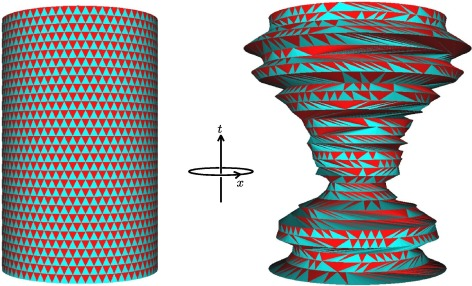
\includegraphics[width=0.75\textwidth]{cdt.jpeg}
\caption{Causal Dynamical Triangulation Microstates[ref]}
\end{figure}

    This approach has shown to be promising in 1+1 and 2+1 dimensions with numerical results agreeing with theoretical models. CDT solves the issue of pertubative non-renormalizability with a discretized spacetime triangulation, where the lattice can be made smaller and smaller to recover the continuous physical limit without blowing up to infinities. 

    \section{Nested Sampling}
    Nested Sampling is an algorithm developed largely by the Astrophysics group at Cambridge. It has many advantages over existing algorithms used for LFT simulations such as Metropolis-Hastings[ref] and Hybrid Montecarlo[ref]. One main advantage is the resistance to topological freezing which occurs near the critical point, an effect where the system gets stuck in local minima and rejection rates of montecarlo methods become very high. This is a well known phenomenon and is an active area of research.

\begin{figure}[H]
\centering
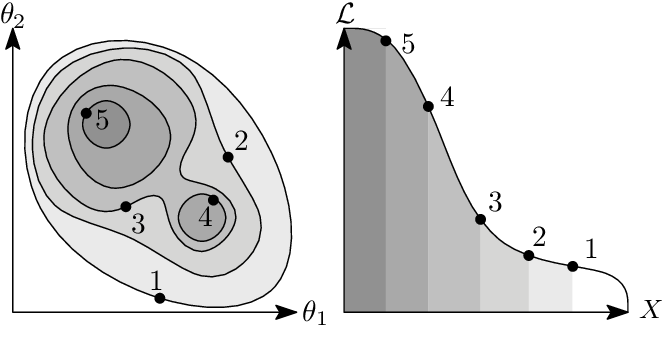
\includegraphics[width=0.75\textwidth]{ns.png}
\caption{Nested Sampling Bimodal Clustering}
\end{figure}

Nested Sampling overcomes topological freezing with its use of clustering and bimodal exploration of a distribution. The challenges involved with applying nested sampling to lattice field theory, and subsequently CDT will relate to the large dimensionality of the models. Every lattice point has multiple parameters associated in the model and must all be explored by nested sampling which itself does not scale well with dimension. These problems will have difficult solutions which will involve careful implementation of computational methods in C++ which have been well tested.

\section{Conclusion}
The application of Nested Sampling to Causal Dynamical Triangulation will be a novel computational approach to Quantum Gravity. The techniques explored will have unique advantages over current methods and will be a valuable research project for the lattice QCD and Quantum Gravity community.


\end{document}
